\clearpage
\section{The `Explore' option}\seclab{Explore}

For the time-calibration we will use a boot-strap method that necessitates the use of some strong pulses for this particular flash. To locate these the program needs to run the script \verb!Explore.sh! (run automatically after RFI-suppression) where the input options are read from the file \verb!"Explore.in"! in the FlashFolder. Typical input lines are

\begin{linenumbers}
\resetlinenumber
\begin{verbatim}
&Parameters
 RunOption= "Explore"
 Calibrations= "Calibrations_ZERO.dat"
! ExcludedStat= "RS210", "RS310", "RS208", "RS409"
 SignFlp_SAI=   21078, 125028, 142092, 142093, 145032, 145033, 166015
 PolFlp_SAI=   021092,  30028,  32092, 106044, 106064, 125028
               145032, 146092, 166014, 181048, 181092,  189076
 BadAnt_SAI=   003065, 021078, 021079, 021093, 026030, 32016, 32017, 32048, 32049
               101045, 125029, 150065, 188051, 188094, 188095
               31086,  31088, 31071
&end
- - - - -- - - -- -
\end{verbatim}
\end{linenumbers}
using the minimal number of input parameters. For the exploratory search of the flash only the antennas within 2.5~km from the core are used.

The program will produce a file in the FlashFolder \verb!"Explore.out"! that has diagnostic information. The script will also produce a plot \verb!"Map_Explore.pdf"! that gives an overview of the image at 30~ms time steps.

\subsection{Figures and print-out}\seclab{Expl-out}

\begin{figure}[th]
\centering{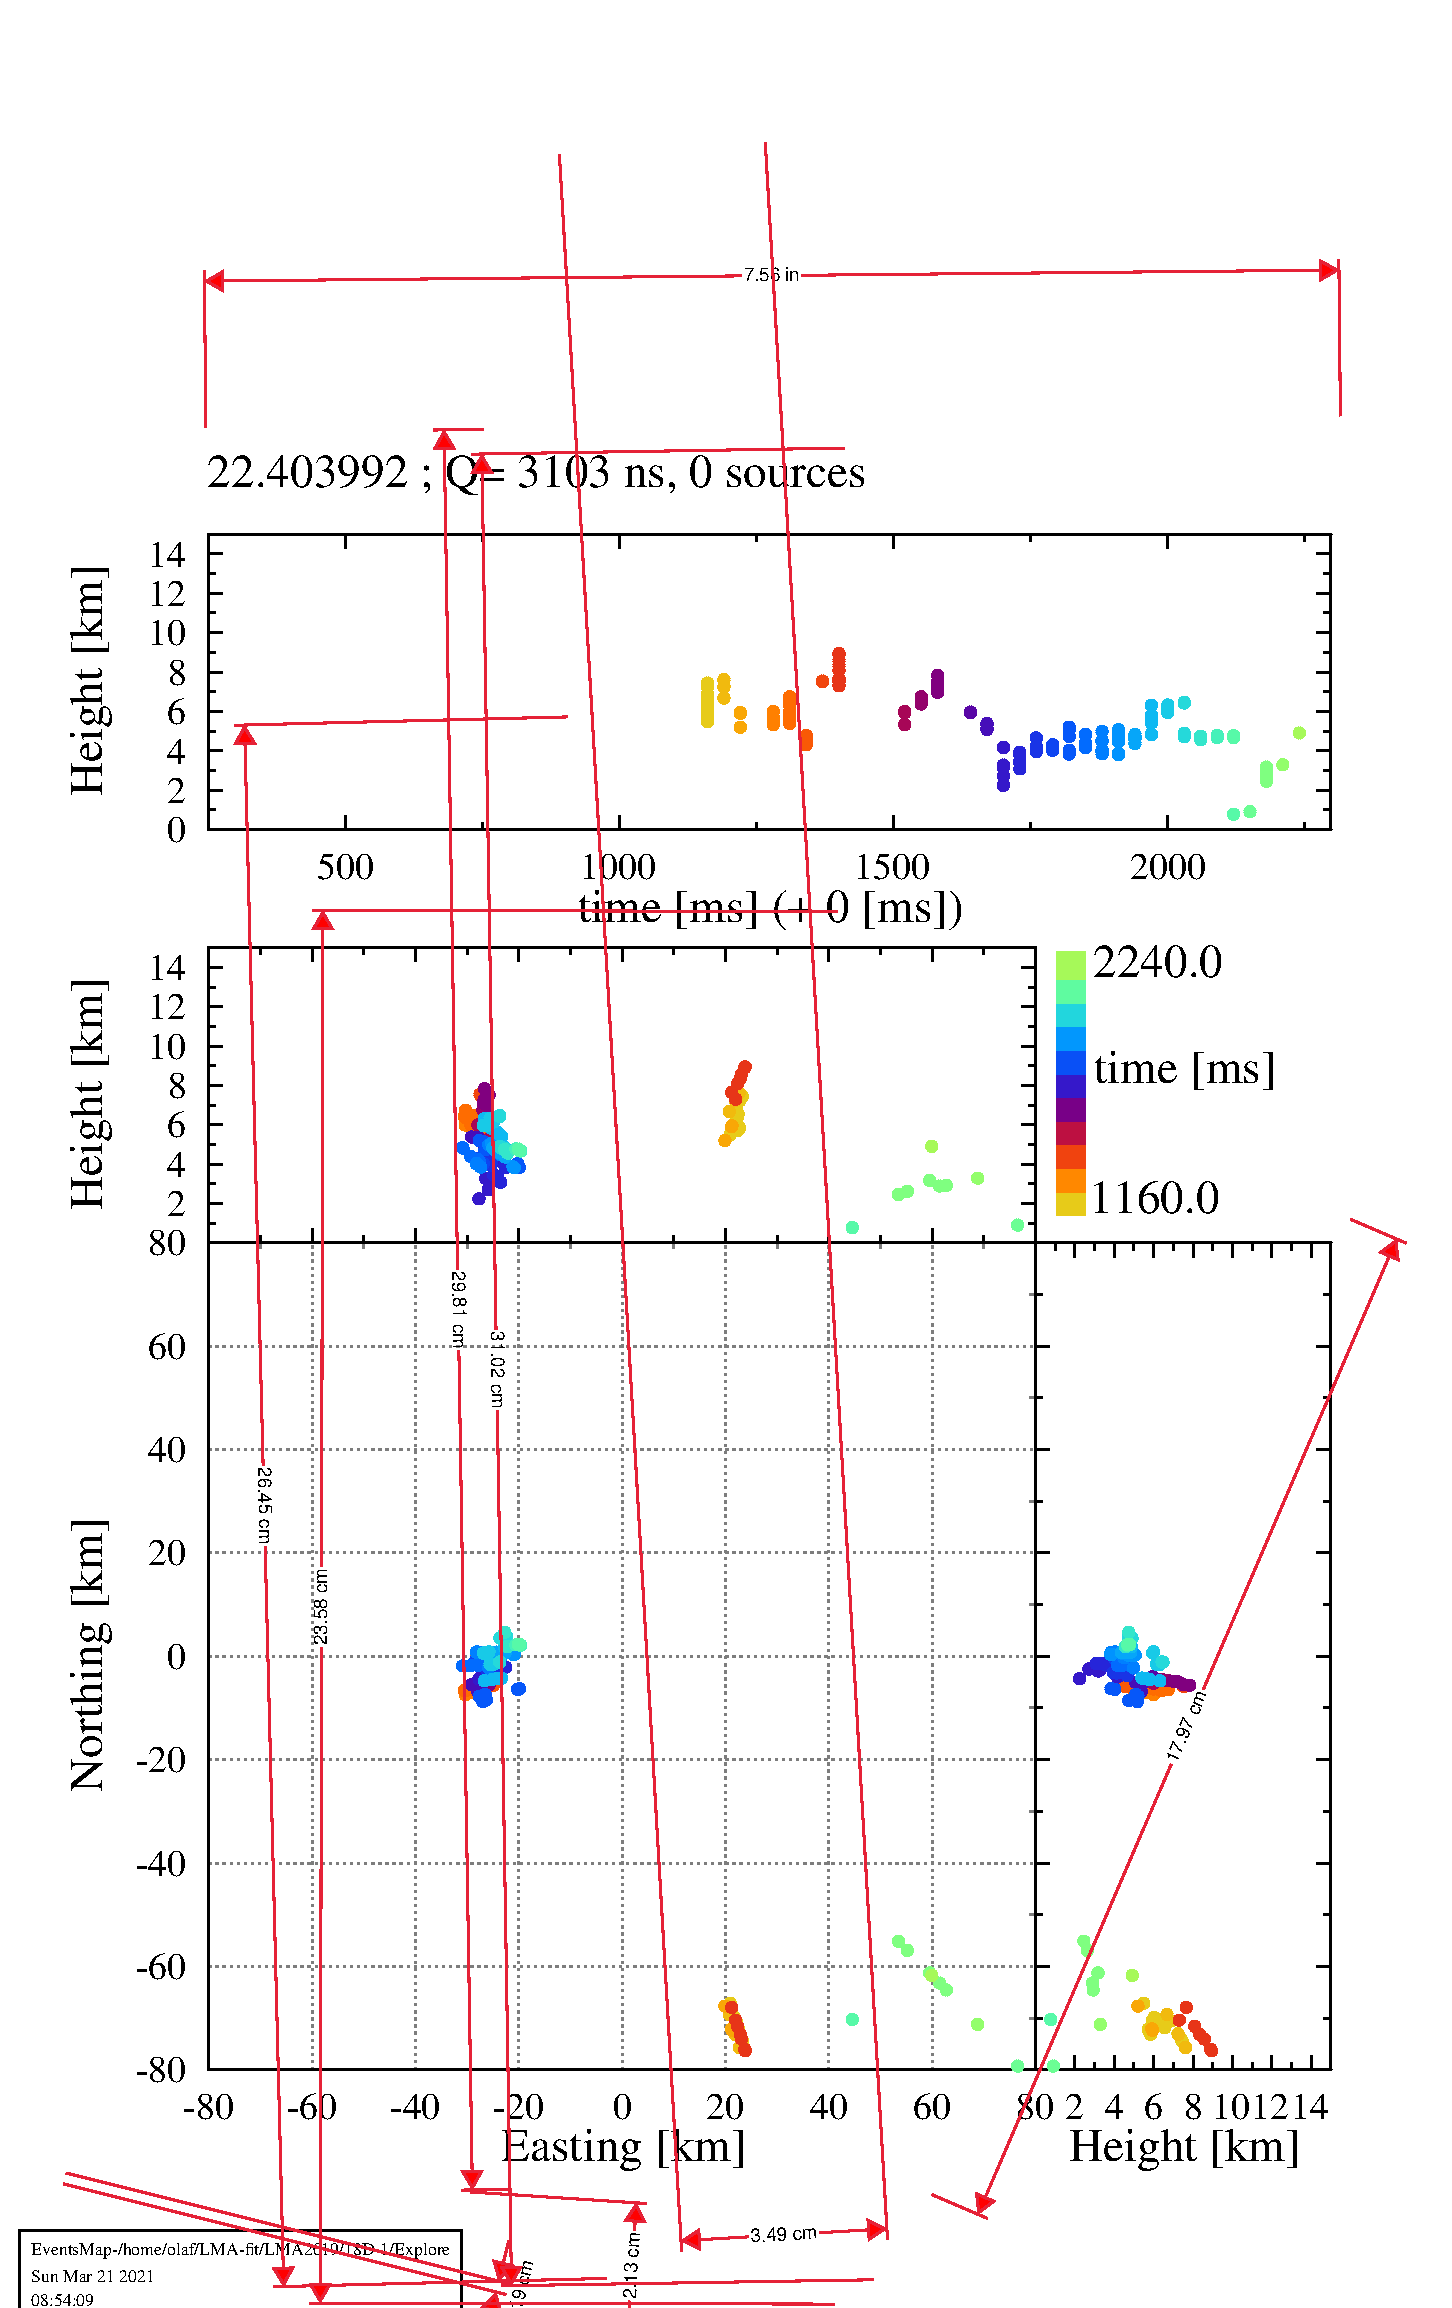
\includegraphics[bb=0cm 0cm 25.5cm 31.4cm,clip, width=0.49\textwidth]{Figs/Map_Explore-18D1} }
%\centering{\includegraphics[ bb=1.0cm 2.4cm 24.5cm 25.7cm,clip, width=0.49\textwidth]{../Figs/SE20A7-NPMx_1HIntfSpecSel} }
	\caption{Exploratory view of Flash 18D1, showing the areas and periods of lightning activity.}	 \figlab{Expl-Fig}
\end{figure}

At the end of the ``explore'' run a plot is made that should resemble \figref{Expl-Fig} giving a rough idea of the spatial and temporal extent of the flash.


